\chapter{Project Planning and Timeline}

\paragraph*{}
For project planning, we have divided the workload into four phases: two for the first semester and two for the second semester. The time allocated for each task is detailed in the attached Gantt Chart, which also specifies the number of group members assigned to each task.

\paragraph*{}
During the first phase, we will focus on simulating our fundamental components: communication, object detection, and SLAM. The communication aspect will explore how robots in a swarm coordinate with one another. Object detection will be implemented using computer vision, and SLAM will have a basic implementation as a proof-of-concept. These simulations will be conducted under the assumption that robots can communicate effectively. All simulations will be conducted using Webots, a robotic simulation platform.This phase is scheduled to take one month.

\paragraph*{}
In the second phase, we will begin integrating hardware by incorporating simple movement. Additionally, we will improve our SLAM implementation. Our primary milestones include testing SLAM in two different environments and implementing an enhanced version of SLAM, such as C-SLAM. These tasks will be undertaken in parallel and are expected to take one month. Once the three group members working on SLAM complete their tasks, they will attempt to combine the individual modules from the first phase into a single simulation. Achieving this integration will result in our Minimum Viable Prototype. This phase aims to be completed by the end of the first semester.

\paragraph*{}
The second semester will focus on gripping and advanced movement, including robot formation. The major milestones for this phase include coordinated gripping, which will test the feasibility of a static gripper for the upcoming sliding movement, and robot formation, which will involve the robots moving together to form a cohesive unit. This phase aims to ensure seamless movement after an object has been gripped.

\paragraph*{}
The final phase will integrate all the functional components developed in simulation with actual robotic hardware. This phase is scheduled to start in February and continue until the project’s completion. Successfully completing this phase will achieve our advanced project goal and ensure that all components function seamlessly in the real world.

\begin{figure}
    \centering
    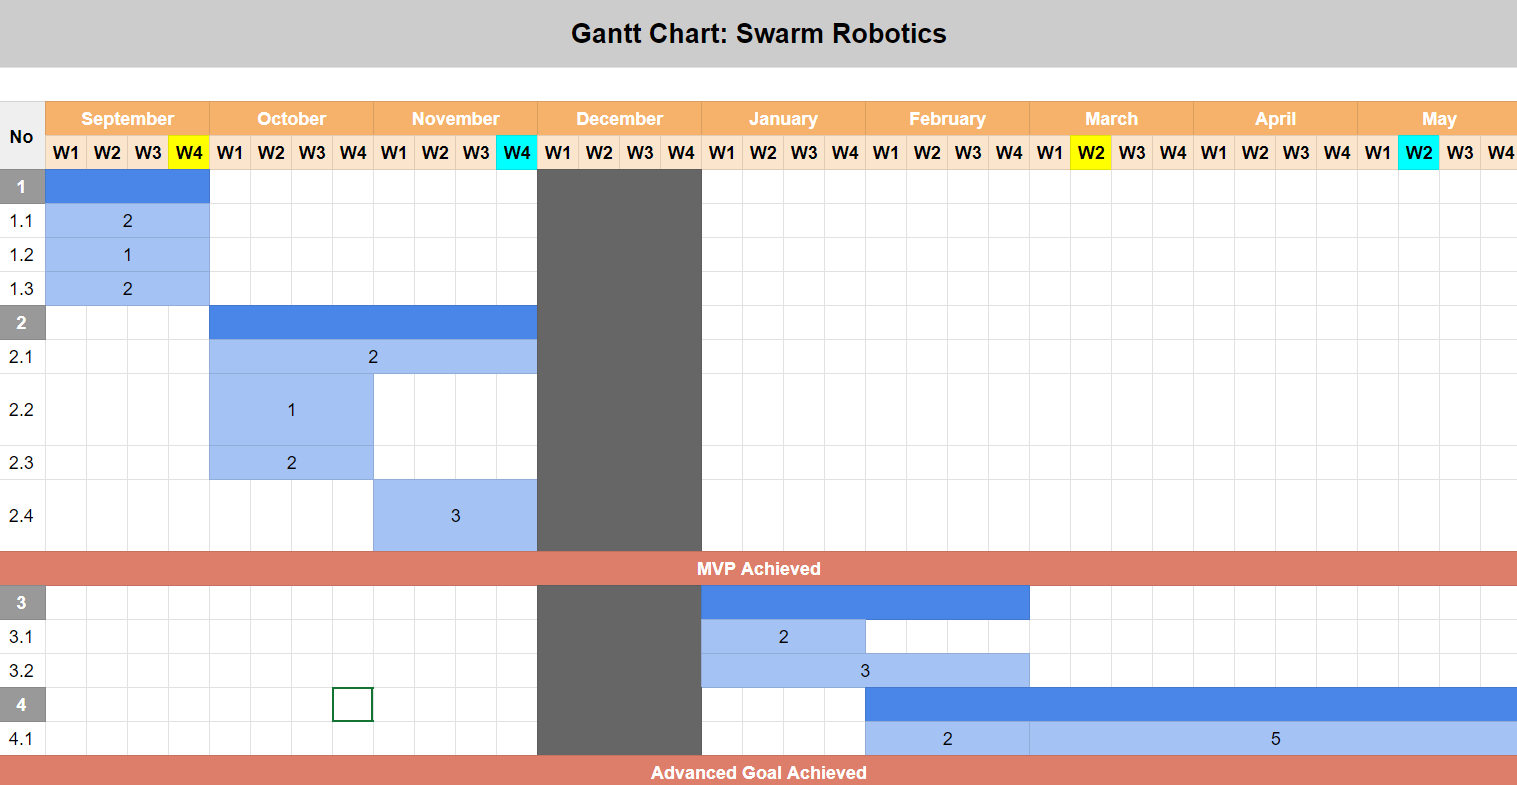
\includegraphics[width=1\linewidth]{assets/images/timeline/gantt_chart.png}
    \caption{Gantt Chart}
    \label{fig:Project Gantt Chart}
\end{figure}

\begin{enumerate}
    \item Simulation
    \begin{enumerate}[label=1.\arabic*]
        \item Communication in the swarm
        \item Object detection using Computer Vision (CV)
        \item Simple Simultaneous Localization and Mapping (SLAM)
    \end{enumerate}
    \item Building the Minimum Viable Prototype (MVP)
    \begin{enumerate}[label=2.\arabic*]
        \item Simple movement with hardware
        \item SLAM in two environments
        \item Improved SLAM
        \item Combine individual modules in simulation
    \end{enumerate}
    \item Coordinated movement with object interactions
    \begin{enumerate}[label=3.\arabic*]
        \item Coordinated gripping with static grippers
        \item Assume swarm formation
    \end{enumerate}
    \item Moving towards the advanced goal
    \begin{enumerate}[label=4.\arabic*]
        \item Combine everything in hardware
    \end{enumerate}
\end{enumerate}
